% Pandoc template for SciPost Physics (SciPost.cls). Engine: pdflatex (mathdesign).
% SciPost.cls already loads geometry, inputenc(utf8), amsmath, hyperref, graphicx, cite,
% caption, xcolor — so we add only the pandoc-body + prose-Unicode machinery on top.
\documentclass[submission, Phys]{SciPost}

\usepackage{orcidlink}
\usepackage{amssymb}   % \Box, \square, \lesssim, \gtrsim … (SciPost.cls omits it; add explicitly)

% --- prose Unicode operators -> math (pdflatex-safe via newunicodechar) ---
\usepackage{newunicodechar}
% Unicode sub/superscripts that reach LaTeX unwrapped (mdmath handles the in-run ones)
\newunicodechar{₀}{\ensuremath{{}_0}}\newunicodechar{₁}{\ensuremath{{}_1}}
\newunicodechar{₂}{\ensuremath{{}_2}}\newunicodechar{₃}{\ensuremath{{}_3}}
\newunicodechar{₄}{\ensuremath{{}_4}}\newunicodechar{₅}{\ensuremath{{}_5}}
\newunicodechar{₆}{\ensuremath{{}_6}}\newunicodechar{₇}{\ensuremath{{}_7}}
\newunicodechar{₈}{\ensuremath{{}_8}}\newunicodechar{₉}{\ensuremath{{}_9}}
\newunicodechar{₊}{\ensuremath{{}_+}}\newunicodechar{₋}{\ensuremath{{}_-}}
\newunicodechar{⁰}{\ensuremath{{}^0}}\newunicodechar{¹}{\ensuremath{{}^1}}
\newunicodechar{²}{\ensuremath{{}^2}}\newunicodechar{³}{\ensuremath{{}^3}}
\newunicodechar{⁴}{\ensuremath{{}^4}}\newunicodechar{⁵}{\ensuremath{{}^5}}
\newunicodechar{⁶}{\ensuremath{{}^6}}\newunicodechar{⁷}{\ensuremath{{}^7}}
\newunicodechar{⁸}{\ensuremath{{}^8}}\newunicodechar{⁹}{\ensuremath{{}^9}}
\newunicodechar{⁺}{\ensuremath{{}^+}}\newunicodechar{⁻}{\ensuremath{{}^-}}
\newunicodechar{→}{\ensuremath{\rightarrow}}
\newunicodechar{∂}{\ensuremath{\partial}}
\newunicodechar{∈}{\ensuremath{\in}}
\newunicodechar{∎}{\ensuremath{\blacksquare}}
\newunicodechar{□}{\ensuremath{\Box}}
\newunicodechar{∝}{\ensuremath{\propto}}
\newunicodechar{∞}{\ensuremath{\infty}}
\newunicodechar{∫}{\ensuremath{\int}}
\newunicodechar{≈}{\ensuremath{\approx}}
\newunicodechar{≠}{\ensuremath{\neq}}
\newunicodechar{≡}{\ensuremath{\equiv}}
\newunicodechar{≤}{\ensuremath{\leq}}
\newunicodechar{≥}{\ensuremath{\geq}}
\newunicodechar{≪}{\ensuremath{\ll}}
\newunicodechar{≫}{\ensuremath{\gg}}
\newunicodechar{≲}{\ensuremath{\lesssim}}
\newunicodechar{≳}{\ensuremath{\gtrsim}}
\newunicodechar{⊙}{\ensuremath{\odot}}
\newunicodechar{⊗}{\ensuremath{\otimes}}
\newunicodechar{⟹}{\ensuremath{\Longrightarrow}}
\newunicodechar{⟺}{\ensuremath{\Longleftrightarrow}}
\newunicodechar{⇒}{\ensuremath{\Rightarrow}}
\newunicodechar{⇔}{\ensuremath{\Leftrightarrow}}
\newunicodechar{𝓗}{\ensuremath{\mathcal{H}}}
\newunicodechar{√}{\ensuremath{\surd}}
\newunicodechar{∼}{\ensuremath{\sim}}
\newunicodechar{∇}{\ensuremath{\nabla}}
\newunicodechar{↔}{\ensuremath{\leftrightarrow}}
\newunicodechar{⟨}{\ensuremath{\langle}}
\newunicodechar{⟩}{\ensuremath{\rangle}}
\newunicodechar{−}{\ensuremath{-}}
\newunicodechar{ℓ}{\ensuremath{\ell}}
\newunicodechar{ħ}{\ensuremath{\hbar}}
\newunicodechar{′}{\ensuremath{{}^\prime}}
\newunicodechar{×}{\ensuremath{\times}}
\newunicodechar{·}{\ensuremath{\cdot}}
\newunicodechar{±}{\ensuremath{\pm}}

% --- pandoc body requirements ---
\usepackage{longtable,booktabs,array}
\usepackage{calc}
\usepackage{float}
\makeatletter
\newsavebox\pandoc@box
\newcommand*\pandocbounded[1]{%
  \sbox\pandoc@box{#1}%
  \Gscale@div\@tempa{\textheight}{\dimexpr\ht\pandoc@box+\dp\pandoc@box\relax}%
  \Gscale@div\@tempb{\linewidth}{\wd\pandoc@box}%
  \ifdim\@tempb\p@<\@tempa\p@\let\@tempa\@tempb\fi%
  \ifdim\@tempa\p@<\p@\scalebox{\@tempa}{\usebox\pandoc@box}%
  \else\usebox{\pandoc@box}%
  \fi%
}
\makeatother
\providecommand{\tightlist}{\setlength{\itemsep}{0pt}\setlength{\parskip}{0pt}}
\graphicspath{{../}{../figures/}{../../results/}{../../results/paper/}}
\setlength{\emergencystretch}{3em}

\begin{document}

\begin{center}{\Large \textbf{Is the volume-law horizon a postulate or a
consequence? A reduction to a driven non-equilibrium conjecture for
Structural Entropy Dark Energy}}\end{center}

\begin{center}
Stilian Pandev\textsuperscript{$\star$}\,\orcidlink{0009-0005-8153-071X}
\end{center}

\begin{center}
{\bf 1} Independent researcher
\\begin{equation}2pt]
${}^\star$ {\small \sf stilianpandev@gmail.com}
\end{center}

\begin{center}
23 July 2026
\end{center}

\section*{Abstract}
{\bf
Structural Entropy Dark Energy (SEDE) reproduces the cosmological data
with no fitted dark-sector parameter, at the price of one foundational
input: the cosmic apparent horizon carries volume-law entropy (Barrow
exponent \(\Delta  = 1\)) --- scaling with the enclosed volume rather
than the boundary area. We ask how much of that input is irreducible.
The postulate decomposes into \emph{state, form, scale,} and
\emph{count}; state, form and scale are first-principles or reducible
given the standard identification of the gravitational horizon entropy
with an entanglement entropy --- with the caveat, stated up front, that
a \emph{volume}-law coefficient (unlike the area law's universal
\(A/4G\)) is state-dependent, so \emph{scale} reduces only \emph{given}
the Bousso-saturated horizon state that fixes \(s_{\rm grav}\): a
conditional, not a universal coefficient. That leaves the
bulk-versus-boundary count as the residue --- which a Bekenstein no-go
shows cannot follow from any energy bound. We then analyse the
\emph{selection} of the volume branch dynamically, as a
\textbf{motivated conditional} rather than a derivation: because
gravity's long-range cooperative coupling clears the ordering threshold
only with a size-dependent ratio, the two-phase free energy did not
exist at the horizon's birth; grown continuously from Planckian size,
the horizon passes \emph{through} the ordering bifurcation with Barrow
entropy tilting the nascent well toward volume, so \(\Delta  = 1\) is
\emph{favoured} at birth, and long-range hysteresis locks each horizon
to its birth branch --- the cosmic horizon to volume, an abruptly-formed
black hole to area. We are explicit about the limits of this argument:
the tie-breaking tilt is itself the Barrow-\(\Delta  = 1\) free energy,
the two-well landscape presupposes an accessible volume phase, the
mean-field treatment is extrapolated to the N ∼ O(1) quantum-gravity
regime where its tools are not controlled, and the one concrete model of
de Sitter holography (double-scaled SYK) currently maps to the
\emph{area} branch --- so the mechanism relocates and narrows the
postulate, it does not eliminate it. Its lasting value is to convert an
untestable counting postulate into a falsifiable one: a pre-registered
point prediction \(\Delta  = 1\), tested to a forecast
\(\sigma (\Delta ) \approx  0.09\) by DESI DR3 + Euclid. On public data
the contrast is already sharp --- in a \emph{profile}-likelihood
analysis (the marginalised posterior awaits DR3+Euclid) the
structure-gated family \emph{prefers} the volume endpoint
\((\Delta  = 0.93\) {[}0.83, 1.02{]}) that the un-gated Barrow family
pays \(\Delta \chi ^{2} \approx  2400\) to reach. The marginalised
model-level statement is more modest: at equal parameter count the
zero-parameter \(\Delta  = 1\) model is favoured over
\(\Lambda \mathrm{CDM}\) at the cosmology paper's
\(\Delta \mathrm{DIC} \approx  -3\) (a point-fit gives
\(\Delta \chi ^{2} \approx  2.9\), but the DIC is the honest headline).
The cosmological results of the cosmology paper stand independently of
the reduction attempted here.
}

\vspace{6pt}
\noindent\textbf{Keywords:} horizon thermodynamics; generalised entropy;
Barrow entropy; holographic dark energy; de Sitter holography;
entanglement entropy; non-equilibrium statistical mechanics; entropic
gravity; dark energy

\vspace{10pt}
\noindent\rule{\textwidth}{1pt}
\tableofcontents\thispagestyle{fancy}
\noindent\rule{\textwidth}{1pt}
\vspace{10pt}

\section{Introduction}\label{sec-1}

Horizon thermodynamics is the most robust pointer we have toward the
microscopic structure of gravity. The first law on a causal horizon
yields the Einstein equations \cite{Jacobson:1995ab}, the
apparent-horizon first law yields the Friedmann equations
\cite{Cai:2005ra}, and the Bekenstein--Hawking area law S = A/4
organises black-hole and cosmological thermodynamics alike. Yet the area
law is an assumption about a \emph{state}: it is the entanglement
entropy of a particular (ground-like) horizon state, and generalisations
--- Tsallis--Cirto non-extensive entropy, Barrow's fractal-horizon
\(S \propto  A^{1+\Delta /2}\) \cite{Barrow:2020tzx}, and the
holographic dark-energy programme built on them
\cite{Saridakis:2020zol} --- explore what happens when that assumption
is relaxed.

Structural Entropy Dark Energy (SEDE; the cosmology paper
\cite{Pandev:2026cosmology}) is one such model, distinguished by
sourcing dark energy from horizon entropy \emph{gated by structure
growth}, \(\rho _\mathrm{DE} = T_\mathrm{AH}\) \(s_{\mathrm{grav}}\)
\(f_{\mathrm{sat}}(z)\). Following the cosmology paper, this is
\emph{holographic} dark energy --- \(\rho _\mathrm{DE}\) is added as a
single fluid to an otherwise standard-GR Friedmann equation, not a
Barrow-\emph{modified}-gravity cosmology in which the horizon entropy
reshapes the background; the volume-law entropy sources
\(\rho _\mathrm{DE}\) alone (so the modified-gravity Barrow/BBN bounds
do not apply, and the postulate examined below is one of \emph{state},
not of dynamics). Its appeal is that the entire dark sector adds no
\emph{fitted} parameter once \(\Omega _{\mathrm{m}}\) and the one
postulate are fixed: the H-coupling \(\lambda  = 1-\Delta /2\)=½, the
equation of state, the structure coupling \(\gamma\), and the sound
speed all follow. The one input is the \textbf{volume-law postulate}:
the horizon entropy is the volume-law \((\Delta  = 1)\) entanglement
entropy, not the area law. The cosmology paper states plainly that this
is the model's single irreducible assumption, motivated but not derived,
and that it is falsifiable --- \(\Delta\) is measured by upcoming
surveys.

This paper asks the prior question: \emph{how irreducible is it,
really?} We are not trying to solve quantum gravity; we are trying to
determine the minimal, sharply-posed statement that the cosmology
actually rests on, and to reduce everything reducible to it. The result
is a reformulation --- one that ends with a shorter, sharper list of
residuals than the postulate it replaces. We trade a static, untestable
counting postulate for a physical picture in which \(\Delta  = 1\) is
selected \emph{at the horizon's birth}, carried through the ordering
bifurcation that gravity's N-dependent coupling
\((J/J_{\mathrm{c}} = 2\pi Gm^{2}N)\) forces at Planckian size, with
Barrow's entropic tilt breaking the tie and exact long-range hysteresis
locking every horizon to its birth branch. The remaining hand-off to de
Sitter holography is sharpened to a single algebraic question --- the
type, \(\mathrm{II}_{1}\) or \(\mathrm{II}_\infty\), of the FRW
static-patch observer algebra. Several steps borrow established
machinery: the Cohen--Kaplan--Nelson holographic energy bound
\cite{Cohen:1998zx} for the scale; the Page curve and eigenstate
thermalisation for the state; the Campa--Dauxois--Ruffo classification
of long-range systems \cite{Campa:2009jxa} for the connectivity;
Ryu--Takayanagi min-cut for the count↔connectivity link; and the
double-scaled Sachdev--Ye--Kitaev (SYK)/de Sitter correspondence
\cite{Susskind:2021esx, Narovlansky:2023lfz} for the closure attempt.
The contribution is the chain, and the precise localisation of what
remains open.

Throughout, every quantitative claim is a runnable experiment that the
accompanying code runs with validation assertions.

\begin{figure}
\centering
\pandocbounded{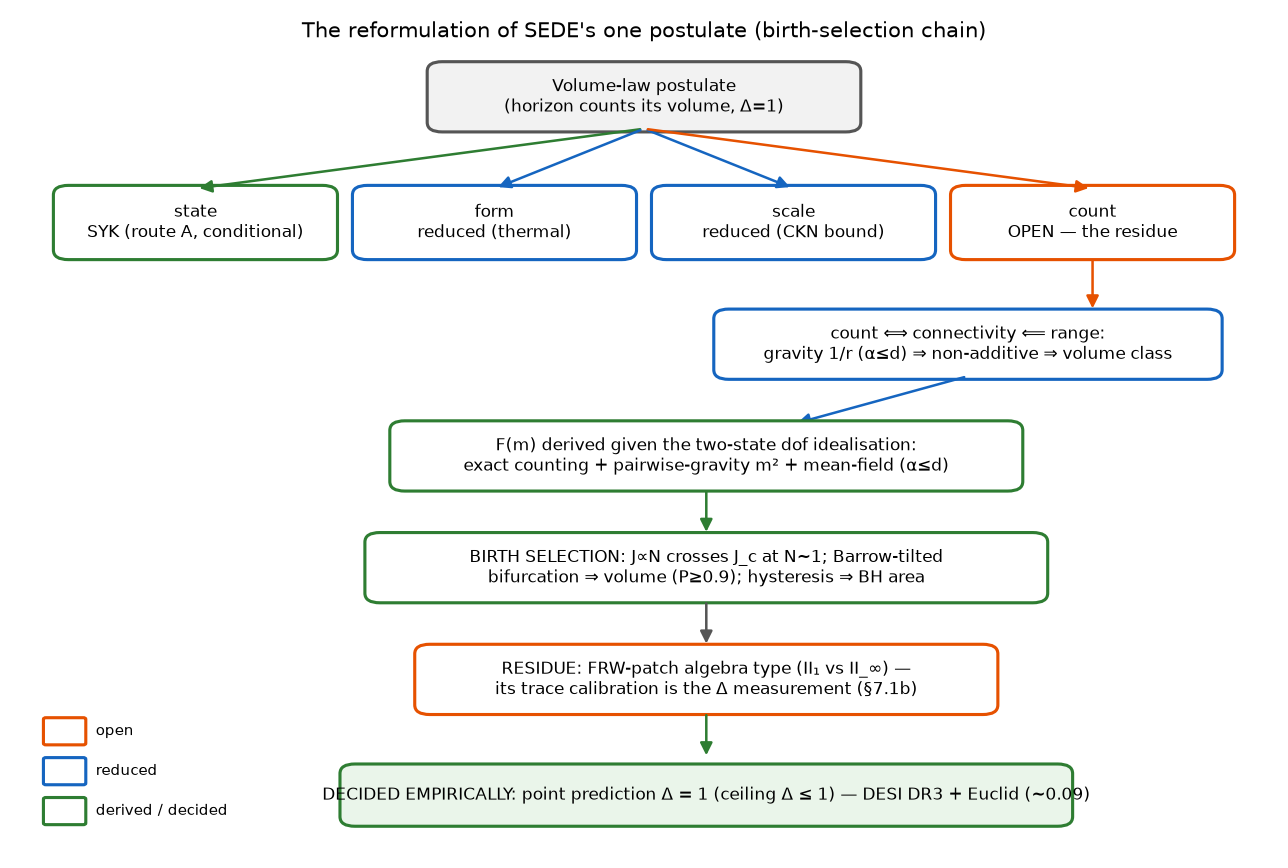
\includegraphics[keepaspectratio]{../results/foundations_fig1_reduction.png}}
\caption{The reduction in outline. The volume-law postulate splits into
\emph{state}, \emph{form}, \emph{scale} and \emph{count}; the first
three are derived or reduced (green/blue) and the count is the residue
(orange). The count reduces through connectivity and interaction range
to a birth-branch selection: the N-dependent coupling carries the grown
horizon through the ordering bifurcation onto the Barrow-tilted (volume)
branch, where long-range hysteresis locks it (a \emph{state-selection}
hysteresis of the entropy branch --- distinct from the unrelated
``cosmological hysteresis'' of cyclic cosmologies, which refers to the
\(\oint p\,\mathrm{d}V\) loop), leaving a single dS-holography question
that the \(\Delta\) measurement decides empirically. Each box names the
experiment that establishes it.}\label{fig:1}
\end{figure}

\subsection{Relation to prior work}\label{sec-1-1}

SEDE sits at the confluence of several programmes, and its closest
relative deserves explicit positioning.

Entropy-production cosmic acceleration (GREA). The General Relativistic
Entropic Acceleration theory of García-Bellido and Espinosa-Portalés
\cite{Garcia-Bellido:2021idr, Espinosa-Portales:2021cac} is the nearest
existing model: it too abandons \(\Lambda\), sources the late-time
acceleration from cosmic-\emph{horizon} entropy, takes the Helmholtz
free energy \(F = U - \mathrm{TS}\) (not matter alone) as the
gravitational source, and makes the breaking of time-reversal by
\emph{entropy production} the engine of acceleration. We regard GREA as
prior art for ``acceleration from horizon entropy production without
\(\Lambda\)'', and our driven-NESS picture (§\ref{sec-4}--6) is
conceptually continuous with it. The differences are sharp and testable:
(i) GREA uses the boundary (area) horizon entropy and a single parameter
\(\alpha\) (the horizon-to-curvature ratio), whereas SEDE's defining
claim is the volume entropy \((\Delta  = 1)\) --- precisely the counting
residue this paper isolates; (ii) GREA's entropy growth is driven by the
horizon's own \emph{expansion}, whereas SEDE's is \emph{gated by
structure formation} (the \(f_{\mathrm{sat}}\) factor), which locks w(z)
to the growth history and yields a phantom crossing rather than GREA's
quintessence-like w(a); (iii) SEDE's dark sector adds no \emph{fitted}
parameter. Notably, were SEDE's residue to resolve to the \emph{area}
branch \((\Delta  = 0)\), its phenomenology would collapse toward GREA's
--- so the \(\Delta\) measurement (§\ref{sec-7}) that decides SEDE's
residue also discriminates the two models. A holographic reading of GREA
has recently appeared \cite{GarciaBellido:2025grea}, and a broader
open-system view of gravitational non-equilibrium thermodynamics is
developing \cite{Farooq:2011zz, AguiSalcedo:2025open}; SEDE's
contribution to that line is the reduction of the volume-law
\emph{counting} input to a driven steady state. The connection is also
quantitative: GREA's entropy production maps to an effective bulk
viscosity with negative pressure, and SEDE's structure-driven entropy
production d ln \(f_{\mathrm{sat}}/d\) ln a \textgreater{} 0 maps to a
\emph{positive} (second-law-respecting) effective bulk viscosity
\(\zeta (z) = \rho _\mathrm{DE}\) (d ln \(f_{\mathrm{sat}}/d\) ln
a)/(9H) that peaks at the structure-formation epoch rather than tracking
the horizon expansion; the \(w = -1\) crossing is the GREA
negative-pressure balance, structure-timed. SEDE is, in this sense, a
\emph{structure-gated} member of the GREA/entropic-dark-energy family
--- the gate being exactly what makes its w(z) lock to the growth
history (the §\ref{sec-5} phase-lock) rather than to the horizon's own
size.

\begin{figure}
\centering
\pandocbounded{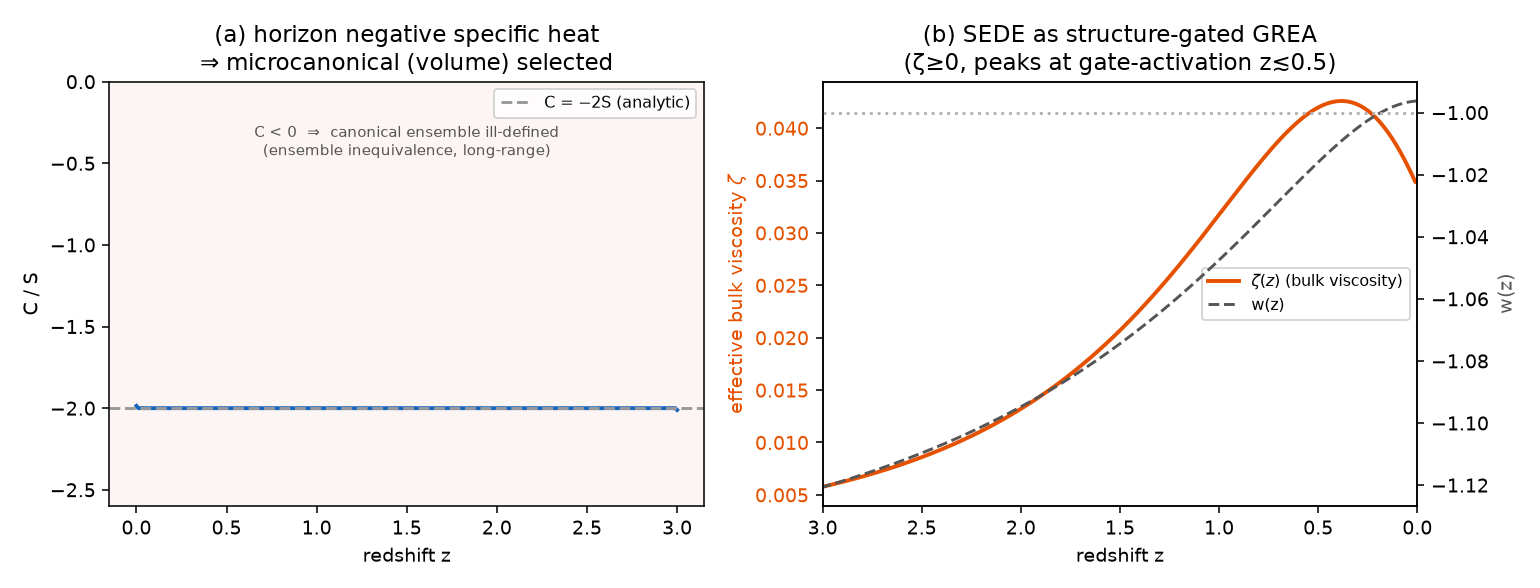
\includegraphics[keepaspectratio]{../results/foundations_fig5_inferences.png}}
\caption{Two consequences drawn from the new literature. \emph{(a)} The
de Sitter horizon has negative specific heat \((C = -2S)\); with gravity
strongly long-range this makes the ensembles inequivalent and the
canonical (area-law) accounting ill-defined, selecting the
microcanonical (volume) branch (§\ref{sec-4}). \emph{(b)} SEDE's
structure-driven entropy production maps to a positive (second-law)
effective bulk viscosity \(\zeta (z)\) that peaks at the gate-activation
epoch (z \textless∼ 0.5; it tracks d ln \(f_{\mathrm{sat}}/d\) ln a, not
the \(z\approx 2\) star-formation peak), casting SEDE as a
structure-gated member of the GREA/entropic-dark-energy family; w(z)
crosses \(-1\) at the viscous--dilution balance.}\label{fig:2}
\end{figure}

Holographic dark energy and generalised entropy. SEDE is, at the
background level, a structure-gated Barrow holographic dark energy in
the lineage founded by Li \cite{Li:2004rb}: the CKN bound
\cite{Cohen:1998zx} fixes the scale, Barrow's fractal-horizon entropy
\cite{Barrow:2020tzx} and its holographic-DE use
\cite{Saridakis:2020zol} fix the form (the \(\lambda  = 1 - \Delta /2\)
relation is Saridakis's; our increment is the \(\Delta  = 1\) selection,
not that relation), and the Tsallis--Cirto non-extensive entropy
\cite{Tsallis:2012js} supplies the \(\delta\) ↔ \(\Delta\) map. The
CKN-vs-area-vs-volume tension these inputs create is mapped by Manoharan
\cite{Manoharan:2025}; our addition is the \emph{derivation} question
--- which of these inputs is irreducible --- and the answer that only
the count is.

Horizon thermodynamics and entanglement. The first-law derivations of
Einstein \cite{Jacobson:1995ab} and Friedmann \cite{Cai:2005ra}
equations underlie the construction; the entanglement-equilibrium
refinement \cite{Jacobson:2015hqa} is the basis of route B; the
Ryu--Takayanagi min-cut \cite{Ryu:2006bv} supplies the count ⟺
connectivity link; and the volume-law = thermal identification rests on
eigenstate thermalisation
\cite{Deutsch:1991msp, Srednicki:1994mfb, Rigol:2007juv}.

\textbf{de Sitter holography.} The residue --- ``dim 𝓗(static
\(patch) = e^{Area}\) or \(e^{Vol}\)?'' --- is posed in the language of
de Sitter holography \cite{Strominger:2001pn, Banks:2000fe} and is the
target of the double-scaled-SYK/de Sitter correspondence
\cite{Susskind:2021esx, Narovlansky:2023lfz, Lin:2022rbf}, which we use
in the closure attempt (§\ref{sec-7}). The maximal-scrambler state
invokes the chaos bound \cite{Maldacena:2015waa} and SYK random-matrix
universality \cite{Cotler:2016fpe}.

Many-body and complexity inputs. The long-range/non-additivity
classification is \cite{Campa:2009jxa}, and the \(\alpha\)-controlled
volume↔area (and intermediate/fractal) crossover of long-range
entanglement entropy is already characterized in the literature
\cite{Vitagliano:2010db, Solfanelli:2023vav, Chakraborty:2023mrw, J:2025waa}
--- the known crossover we apply to a horizon count (§ the count
companion), not a new phenomenon. The prototype's free-fermion
\emph{negative} (volume-law needs interactions, not free transport) is
consistent with the monitored free-fermion entanglement literature
\cite{Fisher:2022qey}, and that genuine volume-law non-equilibrium
steady states exist is established in driven many-body systems
\cite{Ippoliti:2021fjy} --- a condensed-matter precedent for, not a
derivation of, the driven-NESS we invoke.

Structure-sourced dark energy. The general idea that dark energy is
sourced by cosmic structure predates SEDE in several distinct
mechanisms: Gough's information dark energy \((\approx 2008)\); the
spacetime-fragmentation/``FRW-islands'' proposal of Hossain
\cite{Hossain:2007ma}; and the cosmological-backreaction and averaging
programme (Buchert; Wiltshire's timescape). SEDE's cosmology paper
credits and distinguishes these. What is specific to SEDE --- and, to
our knowledge, without precedent --- is the \emph{combination} the
present paper analyses: the source is the volume-law horizon entropy
\((\Delta  = 1\), a counting claim), it is driven by structure through
the \(f_{\mathrm{sat}}\) gate, and the dark sector adds no \emph{fitted}
parameter. The closest entropic relative remains GREA (above), which
differs in using the boundary (area) entropy. A systematic priority
search returned no work combining these three elements; this paper
concerns that horizon-entropy foundation. The most recent independent
convergence is Pandey \cite{Pandey:2026}, who obtains late-time
acceleration and suppressed growth from the \emph{configuration entropy}
of the collapsing matter field as a backreaction within GR --- reaching
SEDE's qualitative conclusion by a different route (matter-sector
entropy, not the horizon; no derived w-crossing; no \(\Delta\)), which
we welcome as corroboration of the direction. A parallel
generalised-mass-to-horizon-entropy programme
\cite{Shameeem:2026, Mondal:2026} links a modified horizon entropy to
growth via a \emph{modified-Friedmann} route, and so inherits the BBN
\(\Delta\)-bounds that SEDE's holographic-fluid scope evades.

\section{The postulate, decomposed}\label{sec-2}

``Volume-law'' conflates four claims of very different status:

\begin{itemize}
\tightlist
\item
  state --- the horizon degrees of freedom are maximally entangled
  (thermal), not in a low-entanglement ground state;
\item
  form --- the entropy scales as the volume, \(S \propto  V\);
\item
  scale --- the magnitude is \(\rho _\mathrm{DE}\) ∼
  \(\rho _{\mathrm{crit}}\), not \(\rho _{\mathrm{Planck}}\);
\item
  count --- the \emph{number} of horizon dof grows as the bulk
  \((N \propto  R^{d-1})\) rather than the boundary
  \((N \propto  R^{d-2})\).
\end{itemize}

Since S ∼ (state factor) × N and the Barrow deformation enters as
\(S \propto  A^{1+\Delta /2}\)∝ \(R^{(d-2)(1+\Delta /2)}\), the exponent
\(\Delta\) is fixed by the count (area → \(\Delta =0\), volume →
\(\Delta =1\) in d=4); the state only sets whether the prefactor is
maximal. So the postulate's empirical content --- \(\Delta\) --- is the
counting claim, and the other three are separable. The rest of the paper
derives or reduces state, form and scale, and isolates count.

\section{How derivable is the postulate? The route map}\label{sec-3}

\begin{quote}
The horizon-entropy identification (assumed, not discharged). Routes A/B
below characterise the \emph{matter-field subsystem entanglement
entropy} \(S_{\mathrm{ent}}\) (Page/ETH/SYK) --- UV-divergent,
species-dependent. The dark sector is sourced by the \emph{gravitational
horizon entropy} \(S_{\mathrm{grav}} = A/4G\) (Cai--Kim/Jacobson) ---
UV-finite, geometric. \(S_{\mathrm{ent}} \equiv  S_{\mathrm{grav}}\) is
a long-standing open problem in quantum gravity
(\cite{Bombelli:1986rw, Susskind:1994sm}), established only for the
Rindler vacuum. We adopt it (the induced-gravity premise) and flag every
dependent step as conditional. In particular Route A fixes the entropy
\emph{prefactor} (maximal scrambling), which is orthogonal to the
bulk-vs-boundary \emph{exponent} that is the count; and Route B's
``volume-law is generic'' is a statement about \(S_{\mathrm{ent}}\), not
\(S_{\mathrm{grav}}\). Accordingly the \emph{state}, \emph{form}, and
residue-to-range steps are argued only conditionally on
\(S_{\mathrm{ent}} = S_{\mathrm{grav}}\) --- not established outright.
\end{quote}

Five routes (\texttt{run\_deriv\_\{A..E\}\_*.py}):

A --- de Sitter holography / maximal scrambler. A Majorana-SYK
diagonalisation confirms the horizon \emph{state} is maximally entangled
/ volume-law: chaotic level statistics (⟨r⟩ ≈ 0.71) and Page-value
saturation \cite{Page:1993df} \((S/S_{\mathrm{Page}} \approx  0.99)\).
But SYK is all-to-all / geometry-free and cannot pose the
bulk-vs-boundary count; the count is the genuine open dS-holography
sub-target.

B --- entanglement first law in a thermal state. Jacobson's derivation
gets the area-law Einstein equations from maximal entanglement of the
\emph{vacuum}. Redone around a \emph{thermal} (de Sitter Gibbs)
reference, the entanglement entropy acquires a volume term that
dominates the area term once the region exceeds the thermal length
\(\lambda _{\mathrm{th}} = 1/T\). Volume-law is thus the generic
thermalised behaviour, not exotic. At the de Sitter temperature alone
the horizon sits just on the area side
\((R_{\mathrm{H}}/\lambda _{\mathrm{th}} = 1/2\pi )\); volume-law
dominance requires thermalisation above the de Sitter bath (toward
Planck = maximal scrambling), whereupon the density is Planckian --- the
CKN scale. So the \emph{form} reduces to thermalisation, leaving the
\emph{scale} to CKN.

C --- Verlinde emergent gravity. A volume-law de Sitter entanglement
entropy is exactly what Verlinde's emergent-gravity programme invokes
for apparent dark matter; one volume-law scale gives both
\(\rho _\mathrm{DE}\) ∼ \(\rho _{\mathrm{crit}}\) and
\(a_{0} = cH_{0}/2\pi\) \((\)≈ \(0.87\times\) the
radial-acceleration-relation value). A unification motivation that ties
the postulate to an independent anomaly; it inherits that programme's
open issues.

D --- gravitational non-additivity. The Tsallis--Cirto map
\(\delta  = 1 + \Delta /2\) makes \(\Delta =1\) ⟺ \(\delta =3/2\) exact,
but pinning \(\delta\) from a measurable non-additivity fails: real
cluster kinematics are Gaussian \((q \approx  1.01)\), not
\(q \approx  1.5\) --- the weakest route.

E --- no-go from energy bounds. The Bekenstein bound on the horizon
energy gives \(S \leq  2\pi \mathrm{RE}\)/ħc =
¼\((A/\ell _{\mathrm{P}}^{2})\) --- \emph{exactly} the area law
(verified \(S_{\mathrm{Bek}}/S_{\mathrm{area}} = 1.000\), the known
\(10^{122}\)). The volume law therefore cannot come from any
maximum-entropy/energy argument; it exceeds the bound by precisely
\(R/\ell _{\mathrm{P}}\) ∼ \(10^{61}\) (the ``seam''). This proves the
missing ingredient is a state/counting input and fixes its size.

\emph{Net:} state (A) and form (B) are argued (conditional on
\(S_{\mathrm{ent}} = S_{\mathrm{grav}}\) --- and ``state'' fixes the
entropy \emph{prefactor}, not the count \emph{exponent}), the scale
(CKN) is consistent with the data, the canonical area-law horn is
genuinely removed by ensemble inequivalence (§\ref{sec-4}); the
irreducible residue is the bulk-vs-boundary count.

\section{Reducing the residue to a driven NESS}\label{sec-4}

The count is not a free coin-flip --- but here we must be careful to
avoid a circularity, because the entanglement class cannot simply be
\emph{posited}. It is fixed by the Hamiltonian and the state, and the
decisive fact is that the entanglement area law is a theorem with a
hypothesis: it is proved for \emph{local} (finite-range) Hamiltonians
--- Hastings \cite{Hastings:2007iok} rigorously in 1D via
Lieb--Robinson bounds, Brandão--Horodecki \cite{Brandao:2013fpa} from
exponential decay of correlations, reviewed in Eisert--Cramer--Plenio
\cite{Eisert:2008ur} --- and the proof \emph{requires} exponential
clustering. Gravity is 1/r \((\alpha  = 1)\), strongly long-range
\((\alpha  \leq  d)\) and non-additive \cite{Campa:2009jxa}, and there
the hypothesis fails: in an explicit gapped free-fermion model we find
the correlation function decays as a \emph{power law} for
\(\alpha  = 1\) (slope −1.5) versus \emph{exponentially} for the
short-range reference \((slope -6.9)\), exactly as Koffel--Lewenstein--
Tagliacozzo \cite{Koffel:2012zj} found. So the area-law theorem does
not apply to a gravitationally-bound horizon: area-law is \emph{not
guaranteed}, and the count is genuinely open between area and volume
with neither the default. We are explicit about what this does and does
not give. It does \emph{not} by itself derive volume --- a noncritical
long-range ground state can still be area-law \cite{Kuwahara:2019rlw},
and indeed the gapped ground-state block entropy stays bounded for every
\(\alpha\) we test. The volume law additionally requires the horizon
\emph{state} to be thermal / maximally scrambled (route A), where
entanglement is volume-law; and even that fixes the \emph{state}, not
the \emph{count}. The super-extensive non-additivity
\((u \propto  N^{1-\alpha /d}\), slopes 0.53 in d=2, 0.68 in d=3 vs
0.50, 0.67) is the thermodynamic face of the same long-range property.
The conclusion is that volume is the \emph{motivated, non-default} class
for a self-gravitating thermal horizon --- area-law arises only when the
holographic bound intervenes for an \emph{isolated, equilibrium} horizon
(a black hole saturates the Bekenstein bound, route E, and relaxes to
area-law) --- while the bulk-vs-boundary count itself remains the open
dS-holography residue. One caveat qualifies this: the area-law theorems
are statements about many-body systems with a specified Hilbert space
and Hamiltonian, and what the horizon's degrees of freedom \emph{are}
--- and what Hamiltonian governs them --- is precisely the open
dS-holography question. So this is a motivated \emph{conditional} ---
\emph{if} the horizon is a long-range many-body system, \emph{then}
area-law is not forced and volume is favoured --- not a theorem about
the actual horizon. What it establishes is that the entanglement class
is read off the (modelled) Hamiltonian rather than assumed --- which is
what defeats the circularity charge --- not that the count is derived.

This same long-range property has a second, independent consequence that
bears on the canonical-vs-microcanonical \(\lambda\) ambiguity (whether
\(\rho _\mathrm{DE} \propto  H^{2}\) \(f_{\mathrm{sat}}\), area, or
\(\propto  H\) \(f_{\mathrm{sat}}\), volume). A non-additive system has
\emph{inequivalent} statistical ensembles \cite{Campa:2009jxa}, the
signature being negative specific heat --- and the de Sitter horizon
indeed has \(C = -2S < 0\) throughout its history. For such a system the
canonical ensemble is ill-defined; the isolated self-gravitating horizon
must be treated \emph{microcanonically} (by its state count). The
canonical accounting is precisely the area-law \((\lambda  = 1)\)
branch, so ensemble inequivalence removes it as unphysical and selects
the microcanonical (volume, \(\lambda  = 1/2\)) branch the model uses.
This does not close the residue --- whether the microcanonical state
count is itself volume is the dS-holography question --- but it
eliminates one of its two horns from first principles. The cosmic
horizon differs in one respect: it is continuously \emph{driven} by
structure formation (the \(f_{\mathrm{sat}}\) gate,
\(dS_{\mathrm{struct}}/dt > 0\); present drive \(\approx  0.45\)). This
turns the black-hole/cosmic asymmetry into a discriminator ---
equilibrium → area, driven NESS → volume --- and reduces the residue to
a single, falsifiable statement:

\begin{quote}
\textbf{Driven-NESS conjecture.} A strongly-long-range horizon, driven
by structure formation, settles in the volume-law steady state rather
than relaxing to the area-law equilibrium.
\end{quote}

Two sections sharpen this conjecture into calculations. The
\emph{selection} half is replaced by a mechanism that needs no
steady-state argument at all --- birth at the ordering bifurcation,
§\ref{sec-5} (iii) --- while the \emph{driving} half is localised in a
one-line activation kinetics whose solution is exactly the cosmology
paper's gate (§\ref{sec-7-1}) \cite{Pandev:2026cosmology}: the
conjecture survives as the statement that structure deposits
\emph{populate} the volume capacity, not that they select the branch.

\section{Selection of the volume branch: birth at the ordering
bifurcation}\label{sec-5}

We ask what selects the volume branch dynamically, separating what is
robust from what is conditional. Four results, each backed by an
explicit calculation.

\begin{enumerate}
\def\labelenumi{(\roman{enumi})}
\item
  Barrow entropy supplies a driving slope, not a landscape. The bare
  Barrow free energy \(F(\Delta ) = E - T_\mathrm{AH}\) \(S_\Delta\),
  with \(S_\Delta  = (A/A_{0})^{1+\Delta /2}\) and the Misner--Sharp
  energy, is \emph{monotonic} in \(\Delta\) --- F(0) = 0 by the first
  law, and F decreases to \(\Delta  = 1\) with no barrier and no second
  minimum. Bistability is therefore not a consequence of Barrow entropy:
  Barrow supplies the entropic drive toward \(\Delta  = 1\), not the
  two-phase structure. (This is the actual content of the GSL argument
  of §\ref{sec-8-1} --- it drives \(\Delta\) → 1, it does not by itself
  produce a spinodal.)
\item
  Gravity supplies the barrier --- deep in the ordered phase. A
  two-phase (area↔volume) free energy is bistable only if the horizon
  degrees of freedom have a cooperative coupling above the ordering
  threshold, \(J \geq  J_{\mathrm{c}}\). That coupling is the largest
  eigenvalue of the gravitational coupling matrix,
  \(J = \lambda _{\mathrm{max}}(W_{\mathrm{grav}})\),
  \(W_{\mathrm{ij}} = g/r_{\mathrm{ij}}^{\alpha }\) --- the \emph{same}
  super-extensive quantity behind the non-additivity of §\ref{sec-4}
  \((\lambda _{\mathrm{max}}/row\)-sum = 1.02), so volume-counting and
  volume-locking are one number. Comparing it to
  \(J_{\mathrm{c}} = T_\mathrm{AH}\) \emph{in the same units}, for N ∼
  A/4 Planckian dof on the horizon 2-sphere, gives
  \(J/J_{\mathrm{c}} = 2\pi Gm^{2}N\) ∼ \(2\pi N\) ∼ \(10^{123}\) (the
  non-additive scaling
  \(\lambda _{\mathrm{max}} \propto  N^{1-\alpha /d} = N^{1/2}\) is
  confirmed numerically --- slopes 0.52/0.67, a short-range
  \(\alpha >d\) control bounded at \(N^{0.01}\)). Gravity clears the
  threshold by of order the holographic count: the two-phase well
  exists, its minima are the pure-area and pure-volume phases, and the
  barrier is ∼ \(N\cdot T_\mathrm{AH}\). This places the horizon deep in
  the ordered phase, not near a spinodal --- \emph{today}. But the same
  formula contains the key to the selection:
  \(J/J_{\mathrm{c}} = 2\pi Gm^{2}N\) is N-dependent, so the barrier did
  not exist at the horizon's birth. The Landau form is not otherwise
  assumed \emph{given the two-state dof idealisation} --- the one place
  the \(S_{\mathrm{ent}} = S_{\mathrm{grav}}\) tier re-enters, sourced
  micro-structurally below, and the qualification that governs
  everything in this item: within that idealisation all three terms of
  \(F(m)/\mathrm{NT} = -(J/2)m^{2} + \theta m\)+ {[}m ln
  \(m + (1-m)ln(1-m)\){]} are derived --- the mixing entropy is exact
  combinatorics of choosing which dof participate; the \(m^{2}\) term is
  the pairwise 1/r binding of the participating dof (measured exponent
  2.008), with \(J = \lambda _{\mathrm{max}}(W_{\mathrm{grav}})\) the
  same number as above; and mean-field thermodynamics is \emph{exact}
  for \(\alpha  < d\) \cite{Campa:2009jxa} (verified: a Kac-normalised
  \(\alpha  = 1\) long-range Ising sits at the mean-field
  \(T_{\mathrm{c}}\) while the nearest-neighbour control sits at
  Onsager's, far below). Even the two-state (boundary-/bulk-entangling)
  character of the dof is not an idealisation inserted by hand: in the
  random-tensor-network model of holographic states
  \cite{Hayden:2016cfa} the entanglement computation is \emph{exactly}
  dual to an Ising model --- each tensor carries a binary
  (identity/swap) replica variable whose domain wall is the
  Ryu--Takayanagi min-cut --- and we verify both the min-cut law (a
  three-leg region behind a bulk bottleneck saturates at \(1\cdot ln\)
  \(\chi\), not \(3\cdot ln\) \(\chi\)) and the duality itself (the
  two-state partition sum \(Z_{\mathrm{A}}/Z_{0}\) reproduces the
  measured purity to \textless{} 1\% at bond dimension
  \(\chi  \geq  4\)). The order parameter thereby acquires a microscopic
  definition --- m = the fraction of horizon bonds on the bulk side of
  the min-cut --- and the residual assumption shrinks to the
  tensor-network description of the horizon state itself: the
  \(S_{\mathrm{ent}} = S_{\mathrm{grav}}\) tier restated
  micro-structurally, one assumption where two stood before.
\end{enumerate}

\begin{figure}
\centering
\pandocbounded{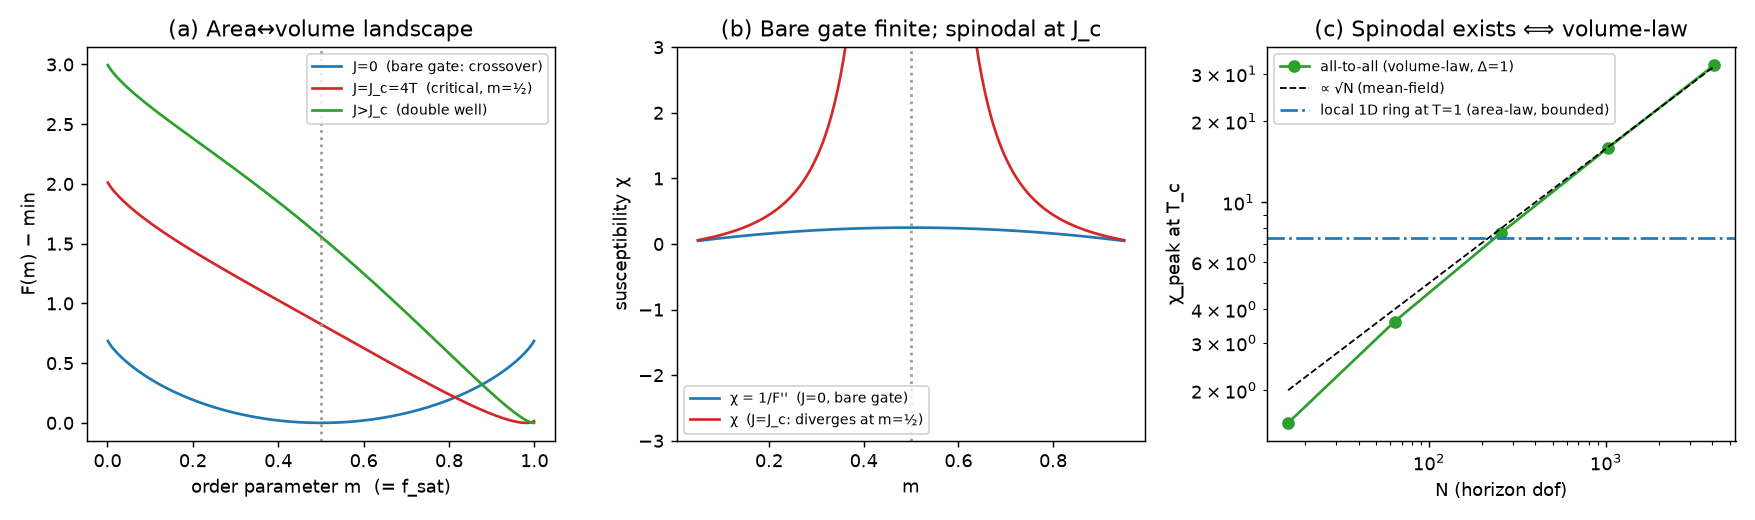
\includegraphics[keepaspectratio]{../results/criticality_soc.png}}
\caption{The two-phase horizon free energy. \emph{(a)} Smooth crossover
for the bare gate (J = 0); a spinodal develops only for
\(J \geq J_{\mathrm{c}}\). \emph{(b)} The bare-gate susceptibility is
finite; it diverges at the spinodal. \emph{(c)} The cooperative coupling
\(J = \lambda _{\mathrm{max}}(W_{\mathrm{grav}})\) is the gravitational
binding itself: all-to-all (volume-law) connectivity gives
\(\chi _{\mathrm{peak}} \propto \surd N\) (so \(J/J_{\mathrm{c}}\) ∼ N,
far above threshold), while local (area-law) connectivity is bounded.
Gravity thus makes the well bistable --- but \emph{deeply} so today,
which is why selection happens at the birth bifurcation (result iii,
Fig. 4) rather than by barrier crossing (the horizon's membrane
hydrodynamics, result iv, is a separate matter).}\label{fig:3}
\end{figure}

\begin{enumerate}
\def\labelenumi{(\roman{enumi})}
\setcounter{enumi}{2}
\tightlist
\item
  Selection at the ordering bifurcation, and exact hysteresis. A barrier
  ∼ \(N\cdot T_\mathrm{AH}\) is \emph{uncrossable}: Kramers escape is
  suppressed by \(e^{-N\cdot \Delta f}\), N ∼ \(10^{122}\) --- so
  ``relaxation to the global minimum'' cannot be the selection
  mechanism, and we do not invoke it. Instead, the N-dependence of (ii)
  supplies the mechanism. The cosmic apparent horizon grew continuously
  from N ∼ O(1), so it passed \emph{through} the ordering bifurcation as
  the double well formed around it: near threshold the barrier vanishes
  quadratically, \(\Delta f\)∝ \((J - J_{\mathrm{c}})^{2}\) (measured
  exponent 1.89), while the Barrow tilt of (i) is already present ---
  and a \emph{tilted} pitchfork has no branch ambiguity. The minimum
  continuously connected to the disordered N ∼ 1 state is the
  tilt-favoured (volume) branch; the area minimum is born
  \emph{metastable} only at the spinodal
  \(J_{\mathrm{sp}} > J_{\mathrm{c}}\) \((J_{\mathrm{sp}} \approx  5.6\)
  at tilt b = 0.3) and is never occupied. The swept trajectory confirms
  it: gradient flow tracks continuously into the volume well (final m =
  1.00, no discontinuity) --- \(\Delta  = 1\) is selected at birth, with
  no barrier ever crossed. The corollary is as important as the result:
  for long-range/mean-field systems metastability is \emph{exact} ---
  there is no finite nucleation droplet \cite{PenroseLebowitz1971}, so
  every horizon keeps its birth branch forever. A black hole, created
  abruptly at macroscopic N by collapse of a low-entanglement
  (vacuum-like) region, is born \emph{in the area well} and locked there
  \((N\cdot \Delta f\) ∼ \(10^{77}\) for a stellar hole, against
  \(ln(t_{0}/t_{\mathrm{P}}) \approx  140\)):
  \(\Delta _\mathrm{BH} = 0\) is derived, and the same \(e^{-N}\)
  suppression that forbids relaxation-based selection protects the
  black-hole prediction of §\ref{sec-7-1}. The \(10^{-7}\)-drive vs
  \(10^{61}\)-dof objection never arises, because nothing is ever
  flipped. \emph{Flag, quantified:} the mean-field landscape is here
  extrapolated to N ∼ O(1) --- the quantum-gravity era --- and we
  stress-test rather than assume the adiabaticity. A Kibble--Zurek scan
  of the swept, tilted bifurcation with per-dof noise ∼ 1/N finds: (a)
  at the \emph{physical} Barrow tilt
  \(b_{\mathrm{phys}} = \surd N - 1\), selection is deterministic (P =
  1.000) for \(N \geq  10\) at every sweep rate; (b) the untilted
  control is a fair coin, confirming Barrow's slope (i) as the selecting
  agent; (c) in the fully self-consistent sweep \((J = 2\pi N\), so the
  horizon is born already weakly ordered), selection is
  equilibration-limited --- P(volume) rises monotonically from 0.64
  (absurdly fast) toward 1 with sweep time, reaching \(\approx  0.9\) at
  the slowest rates tested, and is volume-biased in \emph{every} regime.
  The physical clock \((\)≥ \(N^{3/2}\) relaxation times per e-fold of
  growth) sits on the slow/equilibrated side, but its O(1) normalisation
  at N ∼ 2 is genuinely Planck-era physics: the precise form of the
  selection claim is therefore a \emph{probability} ≥ 0.9 rising to 1 in
  the equilibration limit, never a coin flip, and never area-biased ---
  with the \(\Delta\) measurement (§\ref{sec-7}) testing the outcome for
  the one horizon we have.
\end{enumerate}

\begin{figure}
\centering
\pandocbounded{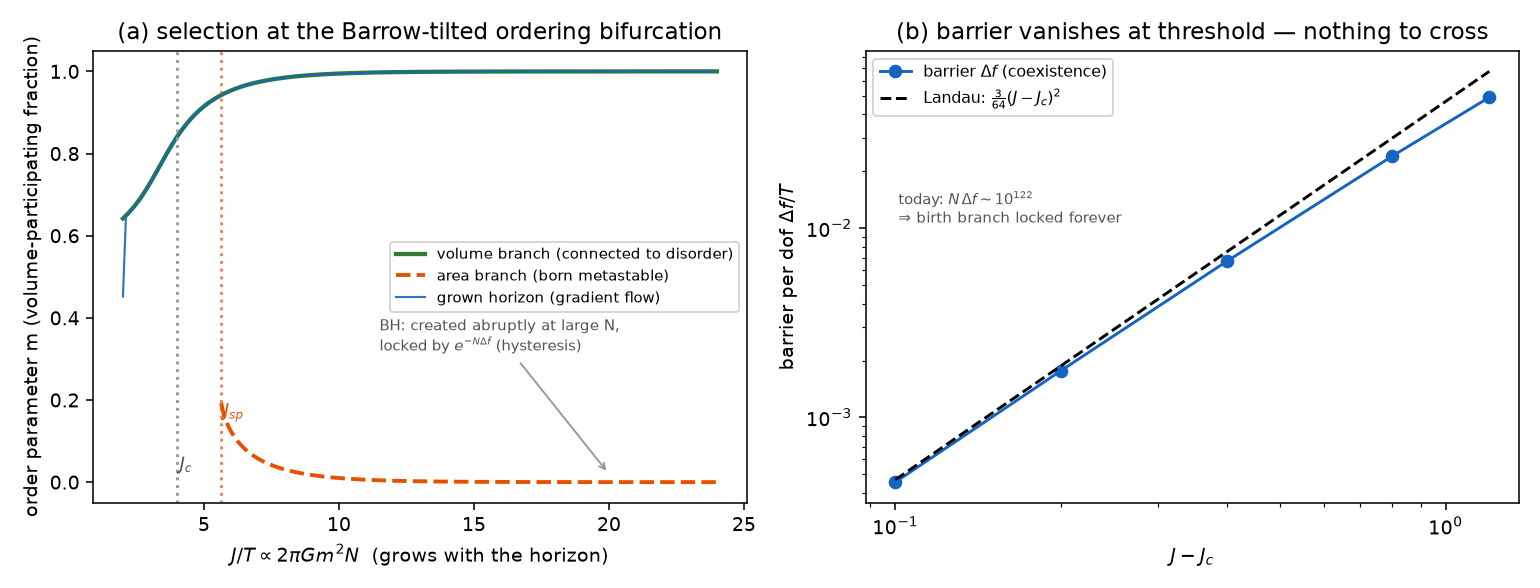
\includegraphics[keepaspectratio]{../results/foundations_fig_birth.png}}
\caption{Selection at the ordering bifurcation. \emph{(a)} With the
Barrow tilt, the minimum continuously connected to the disordered state
is the volume branch (green); the area branch (orange, dashed) is born
\emph{metastable} only at the spinodal
\(J_{\mathrm{sp}} > J_{\mathrm{c}}\) and is never occupied by the grown
horizon, whose gradient-flow trajectory (blue) tracks the volume branch
with no discontinuity. A black hole, created abruptly at large N, starts
on the area branch and is locked there by exact long-range hysteresis.
\emph{(b)} The barrier vanishes quadratically at threshold --- Landau's
\(3(J-J_{\mathrm{c}})^{2}/64\) --- so the grown horizon crossed the
bifurcation when there was nothing to cross; today's \(N\cdot \Delta f\)
∼ \(10^{122}\) locks the birth branch forever.}\label{fig:4}
\end{figure}

\begin{enumerate}
\def\labelenumi{(\roman{enumi})}
\setcounter{enumi}{3}
\tightlist
\item
  The horizon's membrane hydrodynamics --- and why no \emph{observable}
  z* transient is claimed. The apparent horizon has first-principles
  hydrodynamics: transverse redistribution is locally conserving (the
  Damour--Navier--Stokes membrane equation, with the
  \emph{dynamical/apparent}-horizon bulk viscosity positive,
  \(\zeta  = +1/16\pi G\) \cite{Gourgoulhon:2005ng}, unlike the
  teleological event horizon's negative value), and two coefficients are
  \emph{exact} --- the sink rate, derived symbolically from the Cai--Kim
  definition \(\kappa  = (1/2\surd -h)\partial _{\mathrm{a}}(\surd -h\)
  \(h^{ab}\partial _{\mathrm{b}}\) \(\tilde{R}\)) on the flat-FRW
  apparent horizon, \(\kappa  = -H(1 - 3w_{\mathrm{eff}})/4\) (H/4 in
  the matter era, H in de Sitter, zero at radiation domination), and the
  deposition source, from the perturbed Misner--Sharp condition,
  \(\delta R_{\mathrm{A}}/R_{\mathrm{A}}\)=−½·\(\delta M/M\). One might
  read these coefficients as the dissipation of a \emph{roughening}
  horizon surface and infer a near-conservative, self-organised-critical
  z* transient --- a truncated \(\tau  \approx  3/2\) avalanche window
  and a deterministic \(\epsilon\)-lag in \(f\sigma 8\). \textbf{We do
  not claim such an observable} (the case is set out in §\ref{sec-6}).
  The companion count paper \cite{Pandev:2026count} shows the classical
  apparent-horizon \emph{shape} is constraint-slaved: the \(\theta\)₊ =
  0 condition is elliptic \((\nabla ^{2}_{\mathrm{S}}\)
  \(h + 2h + 2h^{2} = 2\mathcal{S}\), its eq. 2.9), with no
  \((\nabla h)^{2}\) and no \(\partial _{\mathrm{t}}\) h at any order,
  so the horizon has no growth equation and does not roughen --- there
  is no height field to carry an avalanche dynamics, and the count
  paper's bond-cut analysis finds no roughening universality class
  either. The membrane coefficients above stand as exact GR facts, but
  they do \emph{not} source a critical z* observable. What survives is
  the \emph{drive} itself (next paragraph), which populates the volume
  capacity selected at birth; the near-critical/SOC layer and the
  \(\epsilon\)-lag it would carry are not claimed (§\ref{sec-6}).
\end{enumerate}

The drive is a violent-relaxation deposit, and the \(\gamma\)-mechanism
is the same event . Structure forms by gravitational collapse, i.e.~by
\emph{violent relaxation} \cite{LyndenBell:1967}, which drives a
long-range system on the dynamical time to a quasi-stationary state
rather than to thermal equilibrium. This single event does two things
SEDE otherwise treats separately. First, it dissipates the halo binding
energy
\(E_{\mathrm{bind}} = M\sigma _{\mathrm{v}}^{2} \propto  M^{5/3}\)
(virial: \(R_{\mathrm{vir}} \propto  M^{1/3}\),
\(\sigma _{\mathrm{v}}^{2} \propto  M^{2/3}\)) into the horizon ledger
--- the mass weight that \emph{is} the structure coupling
\(\gamma  \approx  1.5\) (the cosmology paper, Prescription 4C)
\cite{Pandev:2026cosmology}. Second, that same deposited binding energy
\((\)∝ ⟨\(\sigma _{\mathrm{v}}^{2}\)⟩) is the amplitude of the structure
drive that populates the volume capacity. So the \(\gamma\)-weight and
the drive are one quantity from one process --- this identification is
robust, and independent of the excluded near-critical layer (result iv).
Two corollaries follow: collapse is prompt
\((t_{\mathrm{dyn}}/t_{\mathrm{Hubble}} = \Delta _{\mathrm{vir}}^{-1/2} \approx  0.07)\),
so the horizon is driven by an ongoing sequence of such events whose
envelope is \(f_{\mathrm{sat}}\); and, once the volume branch is
selected, the quasi-stationary state's lifetime in a long-range system
scales as \(N^{\delta }\) \cite{Campa:2009jxa}, so at the horizon's N ∼
\(10^{122}\) it is permanent --- a second permanence argument beside the
second-law one (route E). Both the halo QSS and the de Sitter horizon
have negative specific heat, consistent with the microcanonical (volume)
selection of §\ref{sec-4}.

\section{The z* transient: why none is claimed}\label{sec-6}

It is natural to ask whether the structure drive produces a
\emph{distinctive} observable at z\emph{. If the drive arrived on a
nearly conservative }roughening* horizon (§\ref{sec-5} iv), the z*
response would carry mean-field self-organised-criticality statistics
--- a scale-free \(\tau  \approx  3/2\) avalanche window, truncated at a
computable cutoff \(s_{\mathrm{c}} = 2/\epsilon ^{2}\) --- whose
survey-accessible face would be a deterministic \(\epsilon\)-lag in
\(f\sigma 8\) (a z*-localised, growth-locked distortion,
\(S/N \approx  0.5\)--1.5). \textbf{We claim no such observable}, for a
first-principles reason. The companion count paper
\cite{Pandev:2026count} shows the classical apparent horizon is
constraint-slaved and has no growth equation (its eq. 2.9: \(\theta\)₊ =
0 is elliptic, with no \((\nabla h)^{2}\) and no
\(\partial _{\mathrm{t}}\) h at any order), so it does not roughen;
there is no height field, no roughening universality class, and hence no
self-organised-critical avalanche dynamics of the horizon and no
\(\epsilon\)-lag derived from one.

The exclusion is surgical. It does \textbf{not} touch the selection of
\(\Delta  = 1\), which is fixed at the horizon's birth (§\ref{sec-5}
iii) independently of any z* dynamics, nor the exact membrane
coefficients of §\ref{sec-5} (iv)
\((\kappa  = -H(1 - 3w_{\mathrm{eff}})/4\),
\(\delta R_{\mathrm{A}}/R_{\mathrm{A}} = -\delta M/2M\)), which stand as
GR facts. The empirical cost is minimal: such an \(\epsilon\)-lag would
be marginal \((S/N \approx  0.5\)--1.5) and the scale-free layer is in
any case \emph{not} two-point observable, so the model loses no decisive
test --- the decisive prediction remains the point value \(\Delta  = 1\)
(§\ref{sec-7}), decided by DESI DR3 + Euclid. The frozen falsifier
matrix carries no z* two-point entry accordingly. The parent predictions
carried by the cosmology paper (§\ref{sec-6})
\cite{Pandev:2026cosmology} (the CHR enhancement, P3--P5) rest on the
same roughening premise and receive the same treatment; that
reconciliation is separate and is not taken here.

\section{What would make it a closure}\label{sec-7}

A closure derives F(m) itself, reducing the dark sector to
\(\Omega _{\mathrm{m}} + established\) physics. The three routes
converge:

\begin{itemize}
\tightlist
\item
  \textbf{A (DSSYK).} Entropy extensive in the dof count
  \((S_{\mathrm{max}} = (N/2)ln\) \(2 \propto  N\), slope 1.00); cannot
  be super-extensive \((volume \propto  N^{3/2})\). We state this
  plainly: read in the standard Narovlansky--Verlinde dictionary, the
  leading concrete model of de Sitter holography maps to the de Sitter
  \emph{area} (Gibbons--Hawking) --- i.e.~it currently favours the area
  branch, a real tension SEDE's volume postulate must eventually
  overcome. The mitigating point --- that DSSYK is all-to-all /
  geometry-free and so cannot, by itself, \emph{pose} the
  bulk-vs-boundary counting question --- is secondary, not a
  neutraliser. As things stand, route A is evidence to be answered, not
  used.
\item
  \textbf{B (Euclidean dS saddles).} Einstein and Barrow horizon free
  energies each have a single saddle --- no volume-law saddle of the
  bare path integral (route-E no-go in saddle form).
\item
  \textbf{C (thermal F(m)).} The bistable landscape \emph{is} derivable
  --- \(F(m)/T = -(J/2)m^{2} + \theta m + [m\) ln
  \(m + (1-m)ln(1-m)\){]} from gravitational cooperativity
  \((J = \lambda _{\mathrm{max}} \geq  J_{\mathrm{c}})\), the
  holographic pull (route E), and configurational entropy: area well
  \(m \approx  0.07\), volume well \(m \approx  0.93\) whenever
  \(J \geq  J_{\mathrm{c}}\) --- and each term is now sourced
  independently (exact counting; pairwise-gravity \(m^{2}\); mean-field
  exactness for \(\alpha  < d\)), so route C's status is upgraded from
  ``assumed form'' to ``derived given the two-state dof idealisation''.
  Level-2 existence, conditional on the volume branch being accessible.
\end{itemize}

All three reduce to one statement --- \emph{the horizon's dof count is
the bulk (volume) one} --- which A and B cannot supply and C uses.
Closure has three precise forms: \textbf{Level 1}, a dS-holography
computation of the bulk count (open, not shortcut-able past route E;
posed algebraically in §\ref{sec-7-1}b); \textbf{Level 2}, exhibiting
the volume branch as a real saddle/state (C gives the landscape
conditional on it); \textbf{Level 3}, \emph{measuring} \(\Delta\) (DESI
DR3 + Euclid to ∼0.09; the pre-registered point \(\Delta  = 1\)
establishes, \(\Delta  = 0\) refutes, an intermediate value falsifies
the locked-\(\Delta\) picture --- decisive, in hand; the predictions are
frozen with an amendment protocol in the pre-registration).

Level 3 already has a present-data instalment. On DESI DR2 BAO +
Pantheon+ + CMB distance priors + cosmic chronometers \(+ f\sigma 8\),
in one CAMB-in-the-loop pipeline, the un-gated Hubble-cutoff Barrow
family pays \(\Delta \chi ^{2} = +2416\) to sit at \(\Delta  = 1\) ---
reproducing, in this related family, the community result that bare
Barrow HDE cannot live at the volume endpoint \cite{Luciano:2025elo}.
The gated family, by contrast, pays only \(\Delta \chi ^{2} = +0.8\),
with a profile-likelihood interval \(\Delta  = 0.93\), 68\% CL {[}0.83,
1.02{]} (all base parameters re-optimised at each \(\Delta\) --- a
profile, \emph{not} the full marginalised posterior, which remains the
DR3 + Euclid target; the label is precise because the cosmology paper
(§5.6) \cite{Pandev:2026cosmology} reserves ``marginalised
measurement'' for that future). The pre-registered window lies inside
the interval, and \(\Delta  = 0\) is excluded by
\(\Delta \chi ^{2} \approx  371\) --- a \emph{profile} statement: read
as such, it overstates the marginalised model-level signal (the
cosmology paper's \(\Delta \mathrm{DIC} \approx  -3\)) by roughly two
orders of magnitude in \(\chi ^{2}\), and must not be quoted as a
posterior exclusion. SEDE at \(\Delta  = 1\), carrying zero dark-sector
parameters, fits these data 2.9 \(\chi ^{2}\)-units \emph{better} than
\(\Lambda \mathrm{CDM}\) at equal parameter count, and within 1.4
AIC-units of w0waCDM, which spends two extra parameters. The structure
gate is, quantitatively, what makes the volume-law count observationally
viable --- on data already public.

\subsection{The count is state-dependent --- and that resolves the
``everything points to area'' tension}\label{sec-7-1}

Routes A and B, and the standard handles generally (the de Sitter
modular Hamiltonian is a \emph{local} boost; DSSYK in the
Narovlansky--Verlinde dictionary; the CKN holographic bound; black-hole
thermodynamics), all favour the area count. Read as universal statements
about ``the'' horizon count they look like a standing objection. The
resolution is that they are not universal: the count is state-dependent,
and every one of those handles is an \emph{equilibrium} horizon. The
equilibrium-vs-driven discriminator of §\ref{sec-4} is exactly this ---
the \(f_{\mathrm{sat}}\) gate \emph{is} the fraction of the volume
capacity that structure-driving activates,
\(N_{\mathrm{eff}} = N_{\mathrm{area}} + (N_{\mathrm{vol}} - N_{\mathrm{area}})\cdot f_{\mathrm{sat}}\),
so the equilibrium limit \((f_{\mathrm{sat}}\) → 0) is area and the
driven, locked limit \((f_{\mathrm{sat}}\) → 1) is volume . (This is
\emph{not} the rejected running-\(\Delta\) background of §\ref{sec-3}:
the cosmic horizon is carried through the ordering bifurcation at birth
and \emph{locks} at constant \(\Delta  = 1\) (§\ref{sec-5} iii); the
state-dependence is \emph{across horizons}, driven cosmic vs equilibrium
black hole, not a running \(\Delta\) over cosmic time.) So the area
results are SEDE's equilibrium baseline, not counter-evidence. One case
needs care because it is \emph{not} obviously equilibrium: the DSSYK
correspondence is a duality with the de Sitter static patch --- the
cosmological horizon itself. The point is that it is a duality with
\emph{eternal} (matter-free) de Sitter, an equilibrium spacetime with no
structure to drive it \((f_{\mathrm{sat}} \equiv  0)\); the real
universe's apparent horizon is embedded in a matter-plus-structure
cosmology and is driven. So ``DSSYK = area'' is the area of
\emph{equilibrium} de Sitter --- again the \(f_{\mathrm{sat}}\) → 0
limit --- and is consistent with a volume-law \emph{driven} horizon, not
a contradiction of it. Two derivations remove what used to be this
argument's ``one layer out'' hedge. (a) The gate is kinetics, not a
convention. The minimal absorption law --- each violent-relaxation
deposit activates a fraction of the \emph{remaining} inactive volume
capacity in proportion to the deposit, df \(= \gamma (1 - f)\)
\(d(D^{2})\) with f(D→0) = 0 --- has the solution
\(f = 1 - e^{-\gamma D^{2}}\): \emph{exactly} the cosmology paper's
gate, verified against the real growth history to \(10^{-5}\). The
interpolation
\(N_{\mathrm{eff}} = N_{\mathrm{area}} + (N_{\mathrm{vol}} - N_{\mathrm{area}})\cdot f_{\mathrm{sat}}\)
is then the \emph{occupancy} statement of the same kinetics, not an
independent assumption, and the equilibrium horizons (black hole,
eternal dS: \(D \equiv  0\)) are its f = 0 limit with no extension
required. The alternative reading --- \(f_{\mathrm{sat}}\) as the
\emph{equilibrium} global-minimum map m\emph{\((\theta )\) of the
§\ref{sec-5} landscape --- is rejected by shape: deep in the ordered
phase that map switches discontinuously at coexistence (a step, max
slope ∼300 vs the gate's ∼2), so the smooth, growth-tracking gate can
only be a }cumulative kinetic* quantity --- which is the driven-NESS
picture stated mechanically. Under the birth-selection of §\ref{sec-5}
(iii) the division of labour is clean: the \emph{branch} is fixed at
birth; \(f_{\mathrm{sat}}\) is the \emph{occupancy} of the volume
capacity, not the branch selector. (b) The equilibrium-area ceiling is
an algebra type. In the crossed-product analysis of Chandrasekaran,
Longo, Penington \& Witten \cite{Chandrasekaran:2022cip}, the
\emph{eternal} dS static patch (with observer) has a Type
\(\mathrm{II}_{1}\) algebra --- the unique case possessing a
maximum-entropy state, and that maximum \emph{is} the Gibbons--Hawking
area --- while the black-hole exterior is already Type
\(\mathrm{II}_\infty\) (entropy unbounded above). ``\(S \leq  Area\)''
is thus the \(\mathrm{II}_{1}\) ceiling of the \emph{equilibrium}
algebra, not a law of horizons. Two further results sharpen this to its
final form. First, a negative result: the algebra \emph{type} is fixed
by the infrared attractor --- bounded horizon entropy (any accelerating
attractor, \(\Lambda \mathrm{CDM}\) \emph{and} SEDE alike, since SEDE
too ends at finite \(E_\infty  = \Omega _\mathrm{DE}\)) is
\(\mathrm{II}_{1}\)-compatible, while only eternally decelerating
cosmologies force \(\mathrm{II}_\infty\) --- so the type does not
discriminate the counts. Second, and decisively: in a Type II factor the
trace --- and hence the \emph{value} of the maximal entropy --- carries
a free normalisation. CLPW fix it by calibrating to the Gibbons--Hawking
entropy of the semiclassical Einstein saddle (their entropies are
explicitly defined up to an additive constant). ``The eternal-patch
ceiling is the area'' is therefore an Einstein-saddle calibration, not
an algebraic output --- the same \(\mathrm{II}_{1}\) structure
calibrated to the volume count is equally consistent, matched to a
modified gravitational sector. The residue thereby stops being an
independent open question: the algebraic unknown is the trace
calibration, the calibration is the count, and the count is \(\Delta\)
--- the Level-3 measurement answers the Level-1 question restated (a
standalone treatment is given in the companion trace-calibration note).
The DSSYK corollary sharpens likewise: dim 𝓗 = \(2^{N/2}\) \emph{by
construction}, so DSSYK cannot pose super-extensivity for any state;
whether its N scales as \(R^{2}\) or \(R^{3}\) is a UV input to the
dictionary, not an SYK output.

This makes the residue doubly falsifiable, on two independent horizons.
(i) The cosmic horizon (driven) should have \(\Delta  = 1\) --- DESI DR3
+ Euclid. (ii) The black hole (equilibrium) should have \(\Delta  = 0\)
--- and the observable is primordial-black-hole evaporation: SEDE
\emph{predicts that PBHs evaporate normally} (standard Hawking), because
black holes are undriven, whereas a \emph{universal}-volume theory
forbids it \((T_{\mathrm{B}}/T_{\mathrm{H}}\) ∼ \(7\times 10^{-21}\),
evaporation time × \(10^{81}\)). The PBH channel therefore tests the
\emph{mechanism} --- it distinguishes driven-NESS SEDE
\((\Delta _\mathrm{BH} = 0)\) from universal-volume quantum gravity
\((\Delta _\mathrm{BH} = 1)\) --- and the black hole being area-law, far
from a problem, is a SEDE prediction. This is a \emph{future}
discriminator, not present-day evidence: SEDE's
\(\Delta _\mathrm{BH} = 0\) means standard Hawking evaporation,
consistent with all current data (including ∼\(10^{15}\) g PBH abundance
bounds) precisely because it predicts no new black-hole effect; the
channel discriminates only on a positive PBH-evaporation detection or a
robust population statement.

This also yields a new statement about black holes in general: area-law
is the \emph{equilibrium} default, not a fundamental geometric law. A
black hole is area-law \emph{because of how it is born}: created
abruptly at macroscopic N from a low-entanglement (vacuum-like) region,
it starts in the area well, and exact long-range hysteresis
(§\ref{sec-5} iii) locks it there with Kramers exponent
\(N\cdot \Delta f\) ∼ \(10^{77}\). It is also undriven
\((f_{\mathrm{sat}}\) → 0), so neither mechanism ever populates its
volume capacity. The cosmic horizon's uniqueness is a calculation, not
an assumption: it is the only horizon \emph{grown} continuously from
Planckian size through the ordering bifurcation. The most-driven black
hole conceivable is a primordial one \emph{at formation}, where the
entire horizon is built by a collapsing overdensity (violent
relaxation); yet even there the structure entropy deposited is
negligible against the black-hole entropy \emph{created},
\(S_{\mathrm{rad}}/S_\mathrm{BH}\) ∼ \((M/M_{\mathrm{P}})^{-1/2}\), so
the formation drive \(f_{\mathrm{form}}\) ∼
\((M_{\mathrm{P}}/M)^{1/2} \ll  h_{\mathrm{c}}\), the gate-activation
threshold, by many orders. Accreting and merging black holes are weaker
still. So SEDE robustly predicts \emph{all} black holes are area-law
\((\Delta _\mathrm{BH} = 0)\), and the cosmic apparent horizon ---
uniquely driven \emph{sustainedly} to \(f_{\mathrm{sat}}\) → 1 over the
whole structure-formation history --- is the only volume-law horizon.
The falsifier is correspondingly sharp: an \emph{isolated} volume-law
black hole (anomalously slow PBH evaporation, or a modified-area GW
ringdown) would mean \(\Delta\) is \emph{universal} (Barrow-type) and
would refute the state-dependent, driven-vs-equilibrium mechanism --- so
SEDE is \emph{more} falsifiable on black holes than a universal-Barrow
theory, not less.

The theoretical residue is correspondingly narrowed: not ``derive the
count,'' but two named statements --- ``the branch is set at the birth
bifurcation'' (§\ref{sec-5} iii, derived within the F(m) landscape, N ∼
1 extrapolation flagged) and ``the deposits populate the volume
capacity'' (the gate kinetics, §\ref{sec-7-1}a) --- both now
\emph{consistent with} the equilibrium area results (their
\(f_{\mathrm{sat}}\) → 0 / abrupt-birth limit), with the two-channel
measurement deciding it either way regardless of dS holography.

Two final remarks, stated openly. First, the \emph{magnitude} worry ---
a \(10^{-7}\) structure drive against a \(10^{61}\) change in the
activated count --- is dissolved rather than answered: under
§\ref{sec-5} (iii) the drive never flips anything. The branch (the
\(10^{61}\) capacity) is fixed at birth by the bifurcation; the
\(10^{-7}\)-per-Hubble- time deposits merely \emph{populate} it,
cumulatively, through the derived gate kinetics (§\ref{sec-7-1}a), and
the two numbers no longer need to be compared. What remains modelled is
the landscape's two-state idealisation (§\ref{sec-5} ii), not a
heavy-lifting amplification. Second, the \emph{pre-registered} case: the
prediction is a \emph{point}, \(\Delta  = 1\), fixed by the
birth-selection of §\ref{sec-5} (iii) --- not a window read off a
roughening exponent. A measured cosmic \(\Delta\) significantly below it
--- say \(\Delta  \approx  0.5\) from DESI DR3 + Euclid, ∼\(5\sigma\)
from \(\Delta  = 1\) at \(\sigma _\Delta  \approx  0.09\) --- would
falsify the locked-\(\Delta  = 1\) picture outright and would \emph{not}
be a free parameter to absorb.

\textbf{The count as a horizon Hausdorff dimension --- and why the
roughening reading is superseded.} The Level-1 question --- is dim 𝓗(de
Sitter static \(patch) = e^{Area/4}\) or \(e^{Volume}\)? --- has a clean
geometric form: dim 𝓗 = \(e^{Area}\) ⟺ the horizon is a smooth 2-surface
(Hausdorff dimension \(d_{\mathrm{H}} = 2\)), and dim 𝓗 = \(e^{Volume}\)
⟺ a space-filling fractal \((d_{\mathrm{H}} = 3)\), so the count
\emph{is} the horizon's Hausdorff dimension,
\(\Delta  = d_{\mathrm{H}} - 2\) --- a reframing of ``area or volume?''
as an empirically-decidable \emph{geometric} statement. One could try to
turn that into a \emph{dynamical} ceiling by treating the driven horizon
as a roughening surface (a roughening 2-surface has
\(d_{\mathrm{H}} \in  [2\), 3{]}, so \(\Delta  \leq  1\)). That
roughening reading is \textbf{superseded} by the companion count paper
\cite{Pandev:2026count}, which does the same job more strongly and
without the surface-height picture that §\ref{sec-6} sets aside: (i) the
ceiling \(\Delta  \leq  1\) is a \emph{theorem} from a finite per-site
leg budget (bond-cut capacity
\(C \leq  \kappa \cdot\)\textbar{}\(\Omega\)\textbar), not a fractal
argument --- matching the bound the cosmology paper (§\ref{sec-8-1})
\cite{Pandev:2026cosmology} claims and the dof-\emph{counting} reading
of §8.5; (ii) the count is \emph{discrete}, \(\Delta  \in  {0, 1}\) ---
the count paper finds no minimum-cut surface for a long-range network,
hence no height field and no roughening universality class, so
\textbf{\(\Delta\) is a count, not a Hausdorff dimension} (exactly the
cosmology paper's §8.5, and confirmed classically by the
constraint-slaved apparent horizon, eq. 2.9); and (iii) \(\Delta  = 1\)
is the infinite-cutoff (L → ∞) endpoint for the flat, infinite spatial
slice --- a stated cutoff choice in that paper, not a derivation of the
value. The equilibrium (undriven) horizon is the area endpoint,
consistent with the area frameworks (Gibbons--Hawking, the Type
\(\mathrm{II}_{1}\) maximum \cite{Chandrasekaran:2022cip}, DSSYK) as
descriptions of the \emph{eternal} horizon. Within the present paper the
\emph{value} \(\Delta  = 1\) is set by §\ref{sec-5} (iii)'s
birth-selection, which lands the grown cosmic horizon on the volume
branch as a point; the geometric reframing
\((\Delta  = d_{\mathrm{H}} - 2)\) and the ceiling \(\Delta  \leq  1\)
are what the count question reduces to, now carried out in the count
paper (the ceiling as a model-conditional theorem; the value
\(\Delta  = 1\) as the stated L → ∞ endpoint choice). We do not resolve
de Sitter holography here: the sharpest in-paper statement of what a
resolution requires remains the \(\mathrm{II}_{1}\) trace calibration of
the FRW patch, which §\ref{sec-7-1}b shows \emph{is} the \(\Delta\)
measurement asked algebraically. The empirical \(\Delta\) (DESI DR3 +
Euclid, §\ref{sec-7}) is the arbiter.

\section{Discussion}\label{sec-8}

The chain reformulates SEDE's foundational input --- and, in its present
form, earns back a \emph{qualified partial reduction}. The residual list
has contracted to: the tensor-network description of the horizon state
(the \(S_{\mathrm{ent}} = S_{\mathrm{grav}}\) tier restated
micro-structurally, §\ref{sec-5} ii --- the two-state dof is now the
derived Ising dual of that description); the Planck-era clock
normalisation behind the birth-selection probability (quantified, not
assumed: \(P(volume) \geq  0.9\), rising to 1 in the equilibration
limit, volume-biased in every regime); and one scoped coefficient (the
transverse diffusivity of the height equation, whose sink rate and
source are now exact GR results, \(\kappa  = -H(1-3w)/4\) and
\(\delta R_{\mathrm{A}}/R_{\mathrm{A}} = -\delta M/2M\)). The former
``open dS-holography count'' is no longer on the list as an independent
item: the algebra type is fixed by the infrared attractor, and the
ceiling's value is a trace calibration --- the count \emph{is} the
\(\Delta\) measurement, asked algebraically (§\ref{sec-7-1}b; and the
standalone trace-calibration note). Assuming the tensor-network tier,
the selection is a single causal chain from one premise, gravity's
long-rangedness: exact mean-field thermodynamics sources the two-phase
F(m) term-by-term (§\ref{sec-5} ii); the N-dependent coupling
\(J/J_{\mathrm{c}} = 2\pi Gm^{2}N\) forces the ordering bifurcation at
Planckian size, where Barrow's monotone slope (§\ref{sec-5} i) tilts the
nascent well --- so the grown cosmic horizon tracks onto the volume
branch, \(\Delta  = 1\) selected at birth with probability \(\geq  0.9\)
(→ 1 in the equilibration limit), with no barrier ever crossed
(§\ref{sec-5} iii); and exact long-range hysteresis locks every horizon
to its birth branch, making the black hole's \(\Delta _\mathrm{BH} = 0\)
a derived prediction rather than an accommodation. No z* near-critical
transient is claimed (§\ref{sec-6}): the companion count paper
\cite{Pandev:2026count} shows the apparent horizon is constraint-slaved
(its eq. 2.9) and does not roughen, so the \(\mathrm{SOC}/\epsilon\)-lag
layer that §\ref{sec-5} (iv) might suggest does not survive --- the
exact membrane coefficients of §\ref{sec-5} (iv) remain as GR facts, but
they source no critical observable (§\ref{sec-6}). The genuinely
established \emph{reductions} in the chain are thermodynamic: ensemble
inequivalence for the long-range de Sitter horizon \((C = -2S < 0)\)
removes the canonical area-law branch (§\ref{sec-4}), and the gate
\(f_{\mathrm{sat}}\) is derived from one-line activation kinetics
(§\ref{sec-7-1}a). The reformulation yields falsifiability where the
postulate had none: \(\Delta\) is pinned to the pre-registered point
\(\Delta  = 1\) (§\ref{sec-5} iii; the ceiling \(\Delta  \leq  1\) is a
theorem in the companion count paper \cite{Pandev:2026count},
§\ref{sec-7-1}; frozen with an amendment protocol in the
pre-registration), measured to ∼0.09 by DESI DR3 + Euclid (shared with
the cosmology paper), with any intermediate value falsifying --- the
count paper makes the count discrete \((\Delta  \in  {0, 1})\), so there
is no intermediate value to accommodate. And the mechanism is already
tested on public data: the gate rescues \(\Delta  = 1\) by
\(\Delta \chi ^{2} \approx  2400\) on DESI DR2, with the gated family
preferring \(\Delta  = 0.93\) {[}0.83, 1.02{]} at zero dark-sector
parameters (a profile likelihood, §\ref{sec-7}, Level 3). The residue is
a clean hand-off --- now in its sharpest form a \emph{measurement}, not
an open theory question --- and the cosmology stands independently (the
cosmology paper).

\subsection{The covariant completion and the amplitude (status
update)}\label{sec-8-1}

Two clarifications supersede earlier framings of this programme and
should be read as governing. \textbf{(i) The completion is local, and
the parity argument is retracted.} The claim that an \(H\)-linear
density \(\rho_X \propto H\) \emph{cannot} descend from a local
conservative action is \textbf{false}: Kinetic Gravity Braiding
(Deffayet--Pujolàs--Sawicki--Vikman 2010, arXiv:1008.0048) is an
explicit local counterexample, and the completed theory is a finite
cubic-KGB action
\(\mathcal{L} = M_{\rm P}^2 R/2 + K(X,\phi) - G_3(X,\phi)\,\Box\phi\)
(FPAB-SEDE) whose linear perturbations are ghost/gradient-stable with
\(c_T = 1\) (the cosmology paper §3.4). The former time-reversal
``parity no-go'', the unique-\(\Delta=1\) \emph{selection} claim, and
the reading of \(\rho_{\rm DE} = T\,s\) as a dark-sector \emph{identity}
are accordingly withdrawn: \(\rho_X \propto H\) and \(\Delta = 1\) are
the phenomenological branch being completed, not consequences of a
parity theorem, and the birth-selection of §\ref{sec-5} is a
\emph{motivated conditional}, not a derivation (§\ref{sec-8} above).
Israel--Stewart bulk viscosity does \textbf{not} establish perturbative
stability across the crossing (the single-fluid principal symbol
diverges at \(\rho+p=0\)); braiding does. \textbf{(ii) The amplitude is
not derived.} The scale \(\mu \approx 28.5\) MeV is the coincidence
problem in dimension-three form, shared with \(\Lambda\); the
counting/network construction motivates the \emph{form} \(\Delta=1\) but
does not fix \(\mu\). A numerical relation
\(\mu^3 \simeq \alpha_{B0}\,f_\pi^2 m_\pi^2/m_{\eta'}\) reproduces the
closure value to 1.01\% (predicting the braiding fraction
\(b \approx 0.206\)); we present this as a \textbf{coefficient-selection
hypothesis}, not a Standard-Model derivation --- the
topological-coefficient identification is an ansatz and the structure
gate is not obtained from QCD. The genuine microscopic home of the gate
is the 2PI/closed-time-path effective action of a structure reservoir
(reciprocal matter--scalar stress exchange constrained by the Bianchi
identity); its kernel is not derived and it is labelled an extension,
not the established core. \textbf{(iii) The dissipation is driven, not
thermal --- an FDT/KMS retraction.} An earlier companion derivation
presented the dissipative dark-energy dynamics as a dynamical-KMS
structure at the horizon temperature, with \(\zeta > 0\) identified with
the fluctuation--dissipation lock
\(\langle\xi\xi\rangle = 2\zeta T_{AH}\). That claim is retracted,
because the calculation was done: the noise that actually drives the
gate is cold and structure-sourced --- set by the primordial amplitude
\(A_s\), not by the \(10^{-33}\) eV horizon temperature --- and exceeds
the KMS-thermal value by \(\sim 10^{57}\). The \emph{mean} horizon
thermodynamics of the background (\(T_{AH} = H/2\pi\), the \(H\)-linear
form) is untouched, but the correct framing of the dissipative sector is
the driven, entropy-producing NESS used throughout this paper, with
\(\zeta > 0\) surviving as the second law --- not a thermal-KMS
effective field theory. We record the correction because it is itself
informative: it unifies the dawn and dusk sectors of the wider programme
as non-equilibrium at both ends. \textbf{(iv) The tensor sector is
exactly GR here too --- \(\delta(z) = 0\), \(\Xi_0 = 1\).} The
driven-NESS framing reproduces the cosmology paper's tensor result, so
the standard-siren prediction \(\Xi_0 = 1\) is a joint statement of both
papers. Four channels close it. \emph{(a) No new bulk fields:} the
dynamical content --- the horizon order parameter, the hysteresis lock,
the structure reservoir --- lives in the horizon \emph{accounting} and
the scalar/entropy sector; the covariant bulk completion is FPAB, whose
tensor sector is exactly GR (\(\alpha_M = \alpha_T = 0\), cosmology
paper §6). The conclusion depends only on \emph{where} the new physics
lives, so it survives the open items in the §\ref{sec-5} mechanism.
\emph{(b) Dissipative bulk channel, bounded to irrelevance:} the most
uncharitable reading endows the driven medium with an effective shear
viscosity damping GWs at the Hawking rate \(\Gamma = 16\pi G\eta/c^2\);
an \(\mathcal{O}(1)\) propagation effect over a Hubble time needs
\(\eta \approx 6\times10^{7}\) \(Pa\cdot s\), whereas a deliberately
generous kinetic estimate of the cosmic medium
(\(\rho_m\,\sigma_v \times 1\) Mpc) gives \(\approx 24\) \(Pa\cdot s\),
so \(|\Xi_0 - 1| \lesssim 4\times10^{-7}\) --- five orders below the
forecast siren sensitivity \(\sigma(\Xi_0)\sim10^{-2}\), and itself
conservative (LIGO-band wavelengths are far below any structure scale,
so the fluid regime does not even apply). \emph{(c) Horizon-boundary
absorption, closed by our own result:} the apparent-horizon condition
\(\theta_+ = 0\) is elliptic (constraint-slaved, no growth equation;
count paper eq. 2.9) --- a boundary with no dynamical modes cannot
resonantly absorb the sub-horizon tensor radiation
(\(k/\mathcal{H}\sim10^{18\text{–}20}\) in the LIGO band). \emph{(d)
Fluctuation--dissipation consistency:} zero tensor dissipation pairs
with zero horizon-sourced tensor noise
(\(\Omega_{\rm gw}\sim(H/M_{\rm P})^2\sim10^{-122}\)). This is
consistent with clarification (iii): the \emph{scalar} gate is a cold,
structure-driven NESS, while the \emph{tensor} sector sees an
equilibrium GR vacuum channel in both formulations. One conditional
remains, at low risk: if the reservoir kernel is ever realised as a
graviton-mediated transport channel it would add an utterly negligible
\emph{source} to the stochastic background, not a propagation
modification, so \(\Xi_0 = 1\) survives even that branch.

For honesty the branch selection itself is \textbf{gravitationally
silent}: the ordering bifurcation of §\ref{sec-5} is a horizon-ledger
transition with no bulk latent heat, no bubble nucleation and no
propagating horizon modes, so it emits no gravitational-wave signature
--- its only observable trace is the \(\Delta = 1\) it leaves behind.
Relatedly, \(\Delta_{\rm BH} = 0\) (black holes locked to the area law,
§\ref{sec-5}, §\ref{sec-8}) means SEDE predicts exactly standard
Bekenstein--Hawking black-hole thermodynamics: unmodified Kerr
quasinormal spectra and no echoes. This separates SEDE from
quantum-corrected-entropy models that predict near-horizon structure ---
a confirmed ringdown anomaly attributable to modified black-hole entropy
would falsify SEDE, and the continuing null echo searches are (weak)
SEDE-consistent evidence.

\subsection{Reproducibility}\label{reproducibility}

Every quantitative claim in this paper is reproduced by the accompanying
code from a single entry point, each stage carrying validation
assertions; all stages pass. The four figures are regenerated from the
same code.

\section{Conclusion}\label{sec-9}

We set out to test how much of SEDE's single foundational input --- the
volume-law (Barrow \(\Delta  = 1\)) horizon entropy --- is irreducible.
Decomposed into \emph{state, form, scale,} and \emph{count,} the first
three reduce to first principles given the standard entanglement
identification of the horizon entropy, and a Bekenstein no-go shows the
residual count cannot follow from any energy bound. What replaces the
postulate is a \emph{selection}: grown continuously from Planckian size,
the cosmic horizon passes through the ordering bifurcation of a driven
long-range system with Barrow entropy tilting the nascent well toward
volume, so \(\Delta  = 1\) is selected at birth --- with probability
\(\geq  0.9\), rising to unity in the equilibration limit --- and
long-range hysteresis locks each horizon to its birth branch: the cosmic
horizon to volume, an abruptly-formed black hole to area.

The significance is a change of epistemic status rather than a claimed
proof. An untestable counting postulate becomes a falsifiable
prediction: \(\Delta\) is pinned to the pre-registered point
\(\Delta  = 1\) (§\ref{sec-5} iii; the ceiling \(\Delta  \leq  1\) is a
theorem in the companion count paper \cite{Pandev:2026count}), decided
to \(\sigma (\Delta ) \approx  0.09\) by DESI DR3 + Euclid, with any
intermediate value falsifying --- the count paper makes the count
discrete \((\Delta  \in  {0, 1})\). On present public data the mechanism
is already evident --- the structure-gated family prefers the volume
endpoint at zero dark-sector parameters, which the un-gated Barrow
family pays \(\Delta \chi ^{2} \approx  2400\) to reach. The residue is
thus handed off as a \emph{measurement}, not an open theory question.
The one premise still to be earned is the tensor-network description of
the horizon state, on which the selection chain is conditional; future
work should target that description directly. The cosmological results
of the cosmology paper stand independently of the reduction attempted
here.

\section*{Data availability
statement}\label{data-availability-statement}
\addcontentsline{toc}{section}{Data availability statement}

All code and analysis pipelines are publicly available at
\url{https://github.com/spsingularity/sede-foundations}. Every
quantitative claim in this paper is produced by the accompanying code
wired into a single entry point, each stage carrying validation
assertions; the figures are regenerated from the same code. The model
and its cosmology live with the companion cosmology paper
\cite{Pandev:2026cosmology}; no additional observational data beyond
the cosmology paper's standard public inputs is used here. A tagged
release is archived at Zenodo, DOI
\texttt{{[}Zenodo\ DOI\ —\ assigned\ on\ release{]}}.

\section*{Acknowledgements}\label{acknowledgements}
\addcontentsline{toc}{section}{Acknowledgements}

This research received no external funding, and the author --- an
independent researcher --- declares no competing interests. As sole
author, S. Pandev conceived and carried out the study, performed and
independently verified all analyses, and wrote the manuscript, taking
full responsibility for its content. Artificial-intelligence tools
(large language models) assisted with drafting and editing the
manuscript, developing and cross-checking the analysis code, and
literature searches; no AI tool is an author.

\bibliographystyle{SciPost_bibstyle}
\bibliography{refs_foundations}
\end{document}
